\section{Conclusiones y trabajo a futuro}
En esta sección se presentan las conclusiones obtenidas tras la finalización 
del proyecto, así como las lecciones aprendidas y los conocimientos adquiridos. 
Además, se presentan ideas o propuestas que podrían ser utilizadas o implementadas 
en el futuro para mejorar o ampliar el alcance del proyecto.

\subsection{Conclusiones}
La sección está estructurada en dos partes principales. Primero, se discuten los 
resultados basados en la experiencia directa, evaluando cómo el nuevo stack ha 
reducido los tiempos de desarrollo. Posteriormente, se presentan las opiniones 
y feedback de otros miembros del equipo que han probado y utilizado este stack, 
proporcionando una visión más amplia y diversa sobre su efectividad y beneficios.

\subsubsection{Resultados basados en los desarrollos}
Para evaluar la efectividad del stack tecnológico desarrollado, se realizaron 
varios proyectos de comparando el tiempo necesario para completarlos 
desde cero versus utilizando plantillas y componentes reutilizables. A continuación, 
se presenta una tabla con los tiempos. La tabla \ref{tabla:result-time-scores} 
muestra unicamente el tiempo de desarrollo de los proyectos, sin tener en cuenta
otros factores como el tiempo en la creación de nuevas plantillas o componentes.

\begin{table}[h!]
    \centering
    \begin{tabular}{|l|c|c|c|}
    \hline
    \textbf{Proyecto} & \textbf{Tiempo} & \textbf{Nuevos componentes} & \textbf{Utiliza plantilla} \\
    \hline
    Predicción Temperatura & 3h 30min & 5 & No \\
    \hline
    Consumo Energético & 1h 40min & 1 & Si \\
    \hline
    Clasificación Estación & 2h 00min & 2 & No \\
    \hline
    Estación SKTime & 0h 30min & 0 & Si \\
    \hline
    Anomalías Taxi & 140 & 2 & No \\
    \hline
    Temperatura AutoML & 1h 20min & 1 & Si \\
    \hline
    \end{tabular}
    \caption{Comparación de tiempos de desarrollo de proyectos}
    \label{tabla:result-time-scores}
\end{table}

La utilización de plantillas y componentes reutilizables dentro del nuevo 
marco tecnológico ha demostrado reducir significativamente los tiempos de 
desarrollo de los proyectos. Los proyectos que usaron plantillas, 
presentaron tiempos de desarrollo más bajos en comparación con aquellos que no 
las usaron. Esto sugiere que las plantillas mejora eficientemente y puede ser 
recomendado para futuros desarrollos para minimizar el tiempo invertido en proyectos.\medskip

Otro de los aspectos a destacar es que ha medida que se incorporan nuevos componentes 
al sistema de conocimiento cada vez es más complicado encontrar nuevos que aporten
valor al sistema. Este fenómeno se puede deber a que las necesidades de los proyectos
son bastante similares y los componentes que se han creado hasta ahora cubren la mayoría
de los casos de uso. Por otro lado, es posible que a medida que se vayan incorporando
nuevos miembros al sistema, estos aporten nuevas ideas que permitan la creación de nuevo
conocimiento que no se había contemplado hasta ahora.\medskip

Por último, se ha observado que el uso de técnicas de AutoML ha permitido mejorar
la precisión de los modelos de \textit{forecasting}. Esto se debe a la capacidad de
probar no solo diferentes tipos de algoritmos de \textit{Machine Learning} sino también el uso
de distintas combinaciones de hiperparámetros. 

\subsubsection{Feedback de los usuarios}
Para poder llevar a cabo un análisis de los resultados de la aplicación
de este proyecto, se ha realizado una prueba piloto con un grupo de integrantes
de Tecnalia. Estos han estado probando la herramienta durante un periodo de tiempo
de dos semanas, y han proporcionado feedback sobre su experiencia a través de
la siguiente encuesta de satisfacción.

\begin{itemize}
    \item \textbf{¿La documentación te resultó intuitiva?} 
    
    Esta pregunta busca entender la facilidad de uso y claridad de la documentación proporcionada 
    con la herramienta. La documentación es crucial para que los usuarios puedan 
    aprender a utilizar la herramienta de manera efectiva y rápida, sin tener que 
    buscar ayuda externa constantemente. La figura \ref{fig:sur_1} muestra que el 
    60\% de los encuestados consideran 
    la documentación muy intuitiva, mientras que el 40\% la encuentra 
    mayormente intuitiva. No hubo respuestas indicando que la documentación es 
    confusa. Estos resultados son positivos y sugieren que la documentación es 
    en gran medida clara y fácil de usar se señala que hay áreas que podrían mejorarse. 

    \begin{figure}[!h]
        \centering
        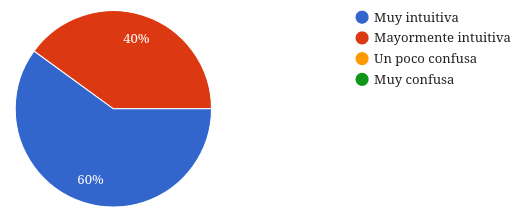
\includegraphics[width=0.65\textwidth]{sur_1.png}
        \caption{Resultado documentación de la herramienta.}
        \label{fig:sur_1}
    \end{figure}
    
    \item \textbf{¿Qué funcionalidad te ha parecido más útil?} 
    
    Se busca identificar cuál de las funcionalidades ofrecidas por la 
    herramienta ha sido la más valorada por los usuarios. Se refire a 
    elementos concretos como los componentes, las plantillas y la gestión de
    experimentos y datasets con ClearML. 

    \begin{figure}[!h]
        \centering
        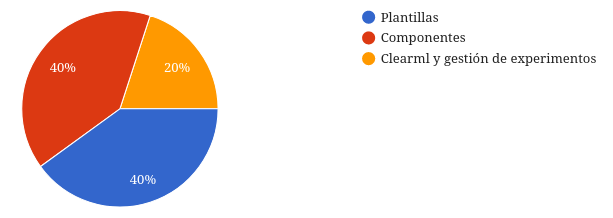
\includegraphics[width=0.8\textwidth]{sur_2.png}
        \caption{Resultado funcionalidades más valoradas.}
        \label{fig:sur_2}
    \end{figure}

    Los resultados indican que las funcionalidades más valoradas por los usuarios son 
    plantillas y componentes, cada una con un 40\% de preferencia, mientras que 
    ClearML es considerada útil por el 20\% de los encuestados. Esto sugiere que, aunque todas 
    las funcionalidades tienen su utilidad, las plantillas y componentes son percibidas 
    como las más valiosas.

    \item \textbf{¿Si tuvieras que contribuir a la documentación, que te gustaría aportar?}
    
    Con esta pregunta se busca entender qué tipo de contribuciones estarían dispuestos
    a hacer los usuarios de la herramienta. Se refiere a la creación de plantillas,
    componentes, entradas de blog, o si por el contrario, no están interesados en contribuir.
    Los resultados indican que el 60\% de los encuestados están dispuestos a contribuir 
    a la documentación mediante la creación de plantillas o componentes. 
    Mientras que otro 40\% no se ven contribuyendo a la documentación y nadie está interesado 
    en contribuir con entradas de blog. Esto sugiere que, aunque hay interés en la creación 
    de plantillas, un porcentaje significativo de usuarios no está dispuesto a contribuir 
    en absoluto. Sería útil investigar las razones detrás de esta falta de interés en 
    contribuir y buscar formas de incentivar la participación, especialmente en áreas como 
    entradas de blog, que pueden ser muy útiles.
    
    \begin{figure}[!h]
        \centering
        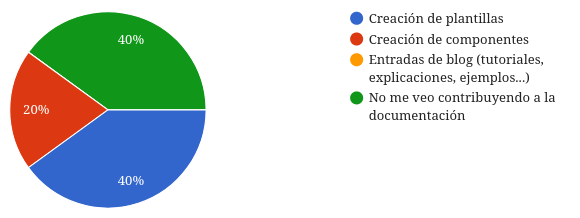
\includegraphics[width=0.8\textwidth]{sur_3.png}
        \caption{Resultado contribución a la documentación.}
        \label{fig:sur_3}
    \end{figure}


    \item \textbf{¿Cuánto tiempo al mes podrías dedicar a contribuir?}

    Con la siguiente cushion se busca medir el compromiso potencial de los usuarios con la 
    herramienta. Se refiere al tiempo que los usuarios estarían dispuestos a invertir 
    en contribuir con feedback, desarrollo, documentación, o cualquier otra 
    forma de colaboración.

    \begin{figure}[!h]
        \centering
        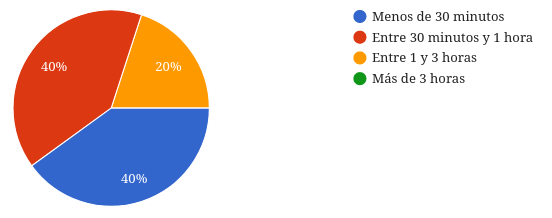
\includegraphics[width=0.8\textwidth]{sur_4.png}
        \caption{Resultado tiempo dedicado a contribuir.}
        \label{fig:sur_4}
    \end{figure}

    Los resultados indican que el 40\% de los encuestados están dispuestos a dedicar menos 
    de 30 minutos al mes para contribuir, y otro 40\% está dispuesto a dedicar entre 30 
    minutos y 1 hora. Un 20\% de los encuestados podría dedicar entre 1 y 3 horas, 
    mientras que ninguno está dispuesto a dedicar más de 3 horas. Esto sugiere que la 
    mayoría de los usuarios tienen un tiempo limitado para contribuir y es importante 
    tener en cuenta este factor al diseñar oportunidades de contribución.
    
    \item \textbf{¿Has utilizado anteriormente alguna plataforma MLOPs?}

    Se investiga el nivel de experiencia previa de los usuarios con plataformas 
    similares de MLOps. Saber si los usuarios tienen experiencia previa ayuda 
    a contextualizar sus respuestas y expectativas. Los resultados indican que el 60\% de 
    los encuestados creen que la herramienta agiliza mucho su trabajo, mientras que el 40\% no 
    la ha utilizado pero le gustaría incorporarla. Estos resultados son muy positivos y sugieren una 
    percepción general favorable de la herramienta. Para aquellos interesados 
    en incorporarla, sería beneficioso proporcionar recursos y apoyo para facilitar 
    su adopción, asegurando así una integración exitosa y mejorando aún más la 
    eficiencia del trabajo.

    \begin{figure}[!h]
        \centering
        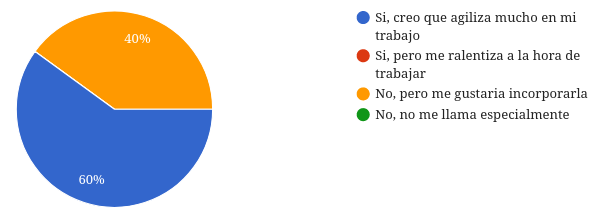
\includegraphics[width=0.8\textwidth]{sur_5.png}
        \caption{Previsualización del componente show\_time\_series\_compare}
        \label{fig:sur_5}
    \end{figure}

    \item \textbf{¿Qué te parece la gestión de datasets de ClearML?} 
    
    Esta pregunta está 
    enfocada en recoger opiniones sobre una funcionalidad específica de la 
    herramienta, en este caso, la gestión de datasets que ofrece ClearML. 
    Se busca entender cómo los usuarios perciben esta funcionalidad en términos 
    de usabilidad.

    \begin{figure}[!h]
        \centering
        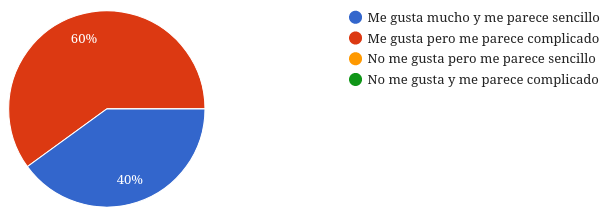
\includegraphics[width=0.8\textwidth]{sur_6.png}
        \caption{Previsualización del componente show\_time\_series\_compare}
        \label{fig:sur_6}
    \end{figure}

    Los resultados indican que el 60\% de los encuestados encuentran la herramienta 
    útil pero complicada, mientras que el 40\% tablen la encuentra útil pero la considera 
    sencilla. Estos resultados sugieren que, aunque la herramienta tiene un valor 
    percibido positivo, su complejidad puede ser una barrera para su uso efectivo. 

    \item \textbf{¿Qué te parece la gestión de experimentos de ClearML?}

    Similar a la pregunta anterior, esta está diseñada para obtener opiniones 
    sobre otra funcionalidad específica: la gestión de experimentos. Se busca 
    evaluar cómo los usuarios perciben la capacidad de la herramienta para 
    gestionar y monitorizar experimentos de machine learning.

    \begin{figure}[!h]
        \centering
        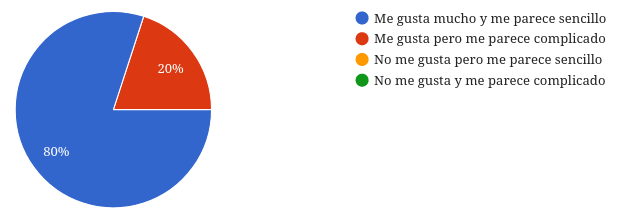
\includegraphics[width=0.8\textwidth]{sur_7.png}
        \caption{Previsualización del componente show\_time\_series\_compare}
        \label{fig:sur_7}
    \end{figure}

    Los resultados indican que el 80\% de los encuestados les gusta mucho la 
    herramienta y la encuentran sencilla de usar, mientras que el 20\% la encuentra 
    útil pero complicada. No hubo respuestas indicando que no les gusta la herramienta, 
    ya sea que la encuentren sencilla o complicada. Estos resultados son muy positivos y 
    sugieren que la gran mayoría de los usuarios están satisfechos con la herramienta y 
    la consideran fácil de usar. Sin embargo, todavía hay un pequeño porcentaje que 
    encuentra la herramienta complicada, por lo que sería beneficioso identificar 
    las áreas específicas que pueden ser simplificadas para mejorar la experiencia de 
    todos los usuarios.

\end{itemize}

\subsection{Trabajo a futuro}
A continuación, se presentan las siguientes propuestas de mejora y ampliación
del proyecto que podrían ser implementadas en futuras iteraciones:

\begin{itemize}
    \item \textbf{Adaptación del sistema a visión por computador:} Actualmente, la infraestructura 
    está enfocada en problemas basados en series temporales, pero se podría ampliar
    su alcance para incluir problemas de visión por computador. Se podría implementar
    no solo funcionalidades de preprocesamiento de imágenes, sino también incluir
    plataformas de etiquetado de imágenes populares como Cvat \cite{CVAT} o incluso conectar el
    sistema de versionado de datasets con herramientas como FiftyOne \cite{FiftyOne}.
    \item \textbf{Integración de ClearML con las tarjetas gráficas de la empresa:} Para 
    optimizar el uso de recursos de cómputo, se propone conectar ClearML con las 
    gráficas (GPUs) de la empresa. Esta integración permitirá gestionar y monitorear las 
    tareas de procesamiento de manera eficiente, asegurando una distribución adecuada de las 
    cargas de trabajo. ClearML facilitará la asignación dinámica de recursos, mejorando 
    la eficiencia del procesamiento y reduciendo tiempos de espera. Se podría implementar un 
    sistema de colas que divida las tareas según su prioridad y requerimientos de recursos. 
    Esto incluiría la creación de diferentes colas para tareas de alta prioridad, 
    tareas de procesamiento intensivo y tareas de mantenimiento. ClearML gestionaría estas colas, 
    asignando las tareas a las GPUs disponibles y asegurando un uso equilibrado y eficiente de los recursos.
    \item \textbf{Monitorización y análisis de rendimiento:} Implementar herramientas de monitorización 
    que proporcionen métricas detalladas sobre el uso de los recursos, el rendimiento de las 
    tareas y la eficiencia del sistema en general. Estas herramientas permitirían identificar 
    cuellos de botella, optimizar la asignación de recursos y planificar mejoras futuras 
    basadas en datos concretos. Además, se podría implementar un sistema de alertas que
    notifique sobre posibles problemas o anomalías en el rendimiento del sistema, permitiendo
    una respuesta rápida y eficaz ante situaciones críticas.
\end{itemize}